\section{Data Analysis}

In this section, we present our results after the execution of sorting algorithms over the input files. We analyzed only the dependent variables \textit{percentage of the largest subarray size ((\%LSS)} and \textit{percentage of unordered elements quantity (\%UEQ)}. These variables, because they are a percentage value, already were normalized (i.e., the same order of magnitude) related to dependent variable array size.

\subsection{Exploratory Data Analysis (EDA)}

Firstly, we performed an analysis of the distribution of the dependent variables \%LSS and \%UEQ. To help in this task, we produced histograms, boxplot graphs, tables containing data about mean, median, standard deviation, and the minimum and maximum values.

The following Figures \ref{fig-histogram-boxplot-bubble-001100}, \ref{fig-histogram-boxplot-insertion-001100}, \ref{fig-histogram-boxplot-merge-00510000} and \ref{fig-histogram-boxplot-quick-00510000} illustrates examples of histograms and boxplot graphs for each combination of \textit{Algorithm X Probability of Failure X Array Size}. In each of those figures, the graphs were exhibited over the dependent variables \%LSS and \%UEQ.  In the histogram, the red vertical line means the mean, and the blue vertical line means the median. On the other hand, in the boxplot, the red horizontal line means the mean, and the blue horizontal line means the median.

\begin{figure}[H]
    \centering
    \frame{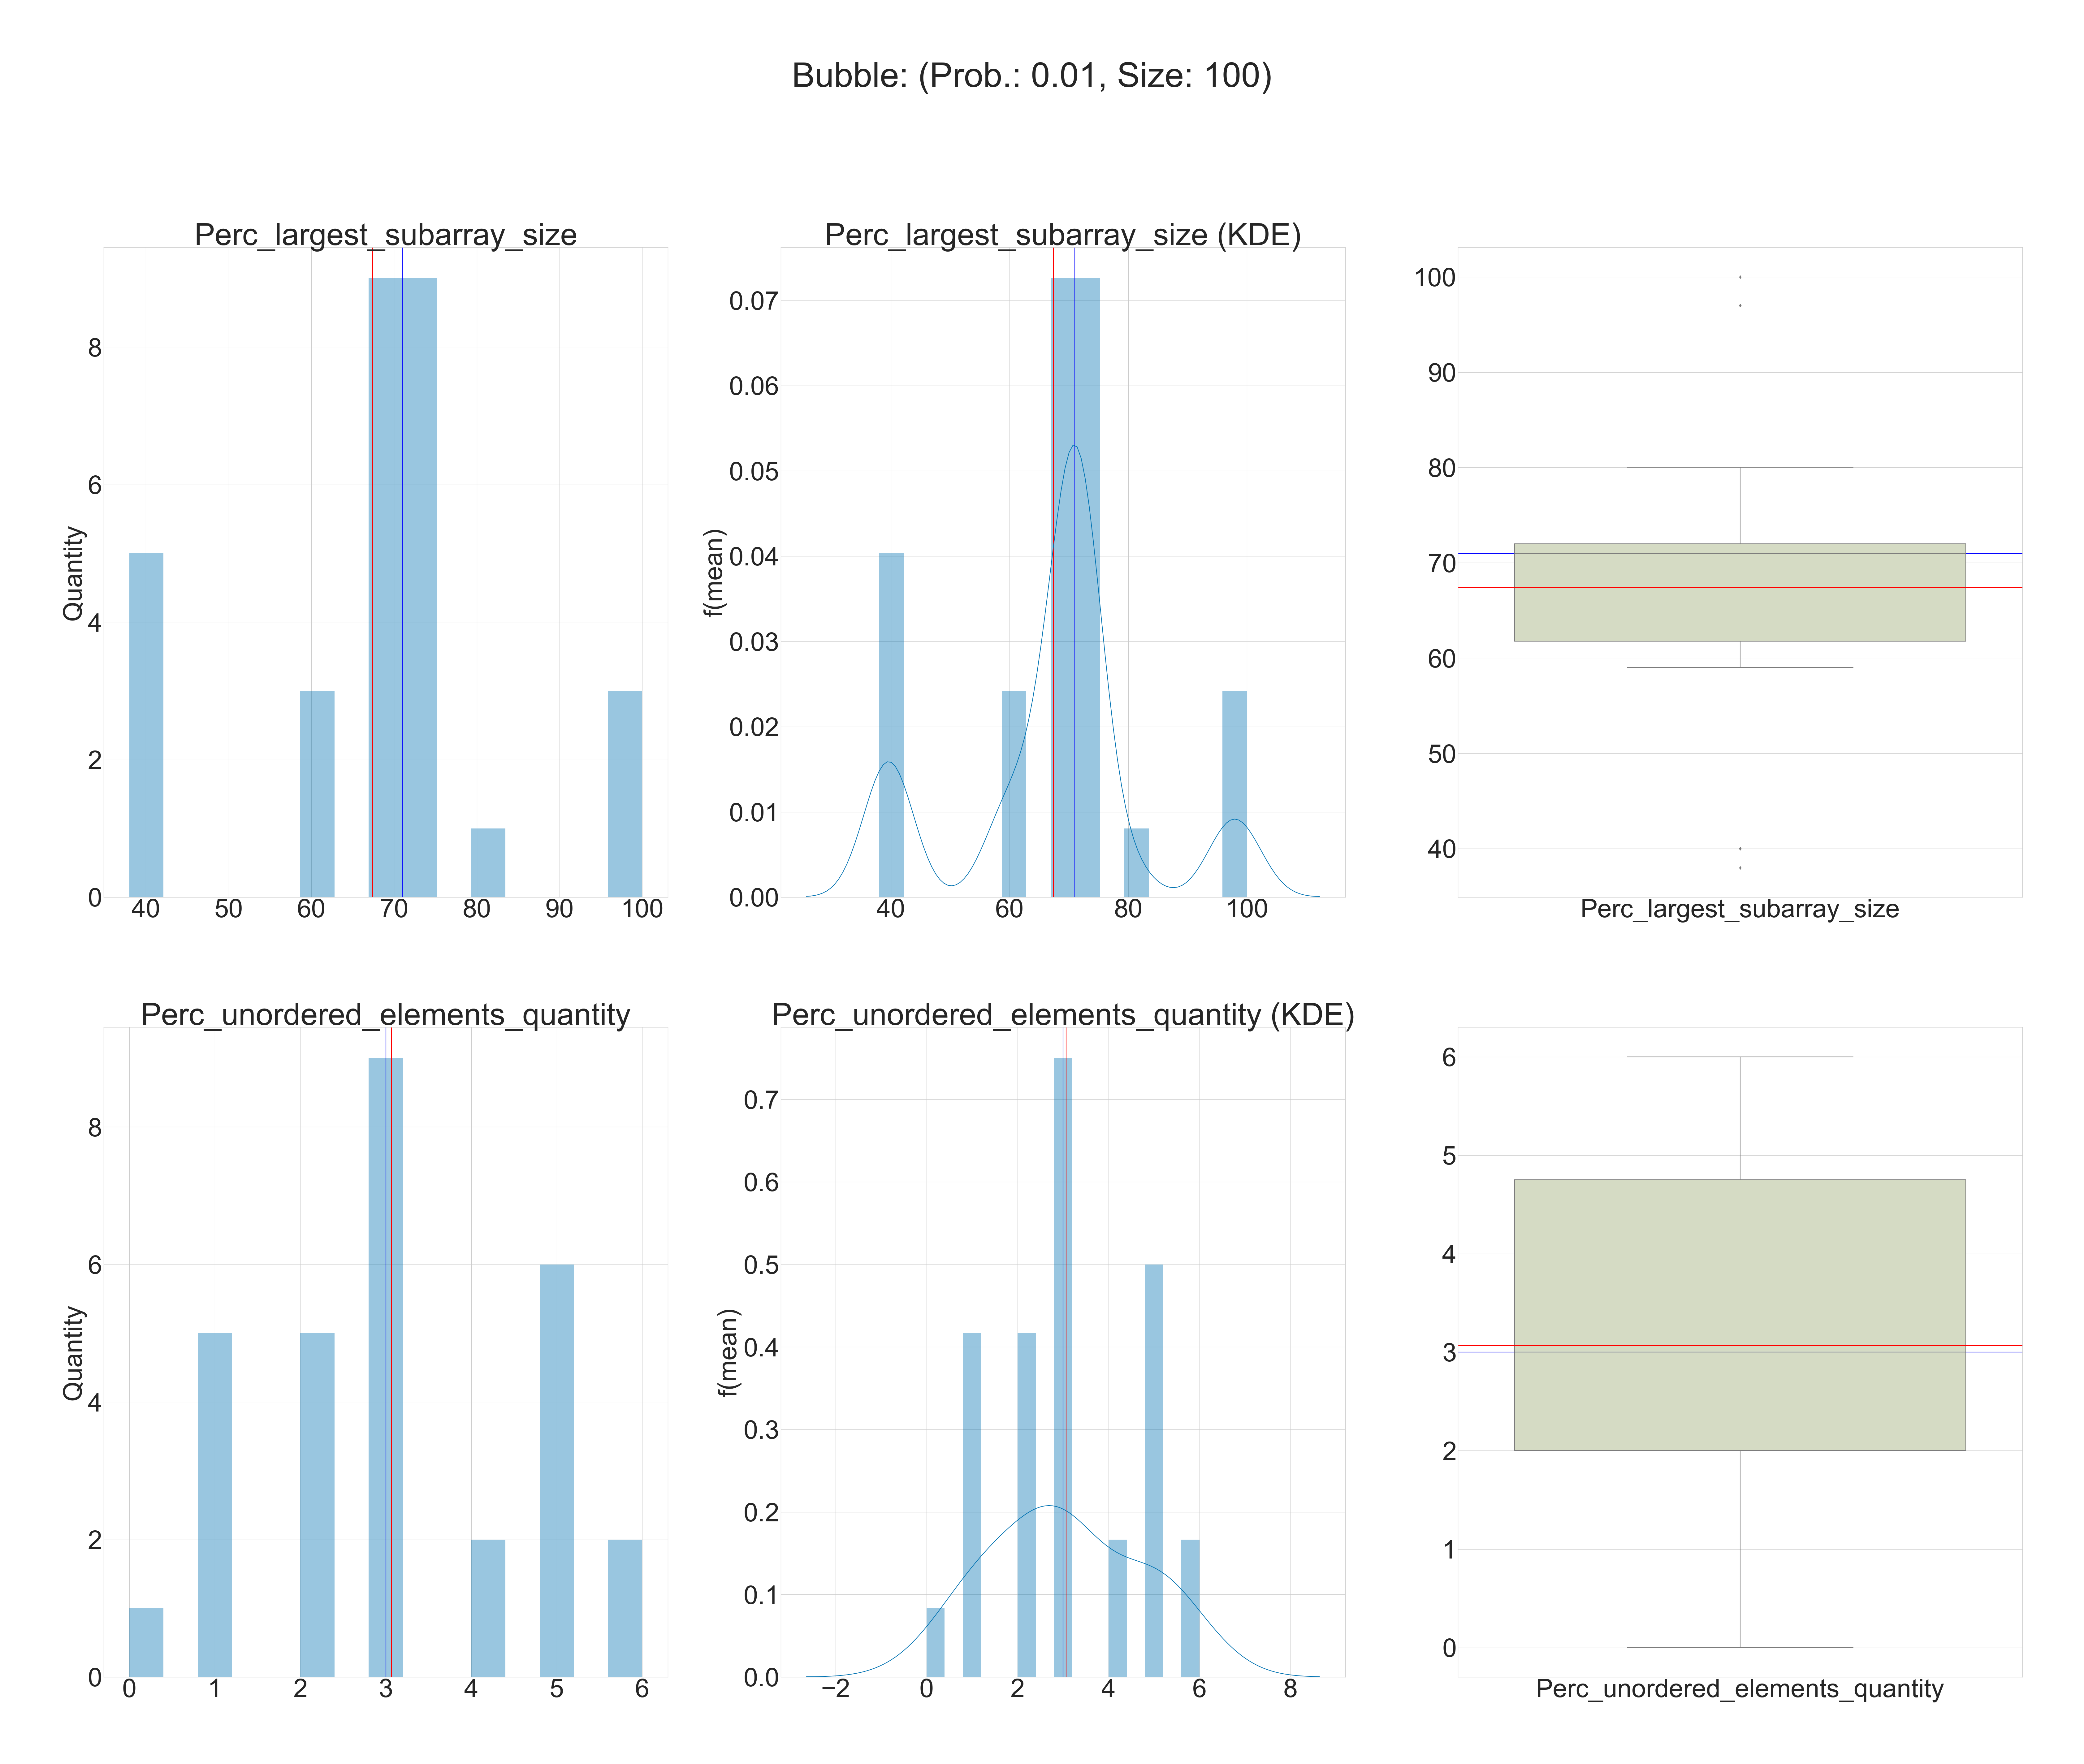
\includegraphics[scale=0.105]{figures/0_01_100_Bubble.png}}
    \caption{Histograms and Boxplot for Bubblesort, with \textit{probability of failure} of 0.01 and \textit{array size} of 100.}
    \label{fig-histogram-boxplot-bubble-001100}
\end{figure}

Based on Figures \ref{fig-histogram-boxplot-bubble-001100}, \ref{fig-histogram-boxplot-insertion-001100}, \ref{fig-histogram-boxplot-merge-00510000} and \ref{fig-histogram-boxplot-quick-00510000}, the following tables illustrates the information about the dependent variables (\%LSS and \%UEQ) distribution.

\begin{table}[H]
    \caption{Table Type Styles}
    \begin{center}
    \begin{tabular}{|c|c|c|c|c|}
    \hline
    \textbf{Prob. of Failure} & \textbf{Array Size} & \multicolumn{3}{|c|}{\textbf{Table Column Head}} \\
    \cline{2-4} 
     & \textbf{\textit{Table column subhead}}& \textbf{\textit{Subhead}}& \textbf{\textit{Subhead}} \\
    \hline
    copy & adsad & asdasd & asdasd \\
    \hline
    \end{tabular}
    \label{tab-distribution-depentent-variable-ueq}
    \end{center}
\end{table}

\begin{figure}[H]
    \centering
    \frame{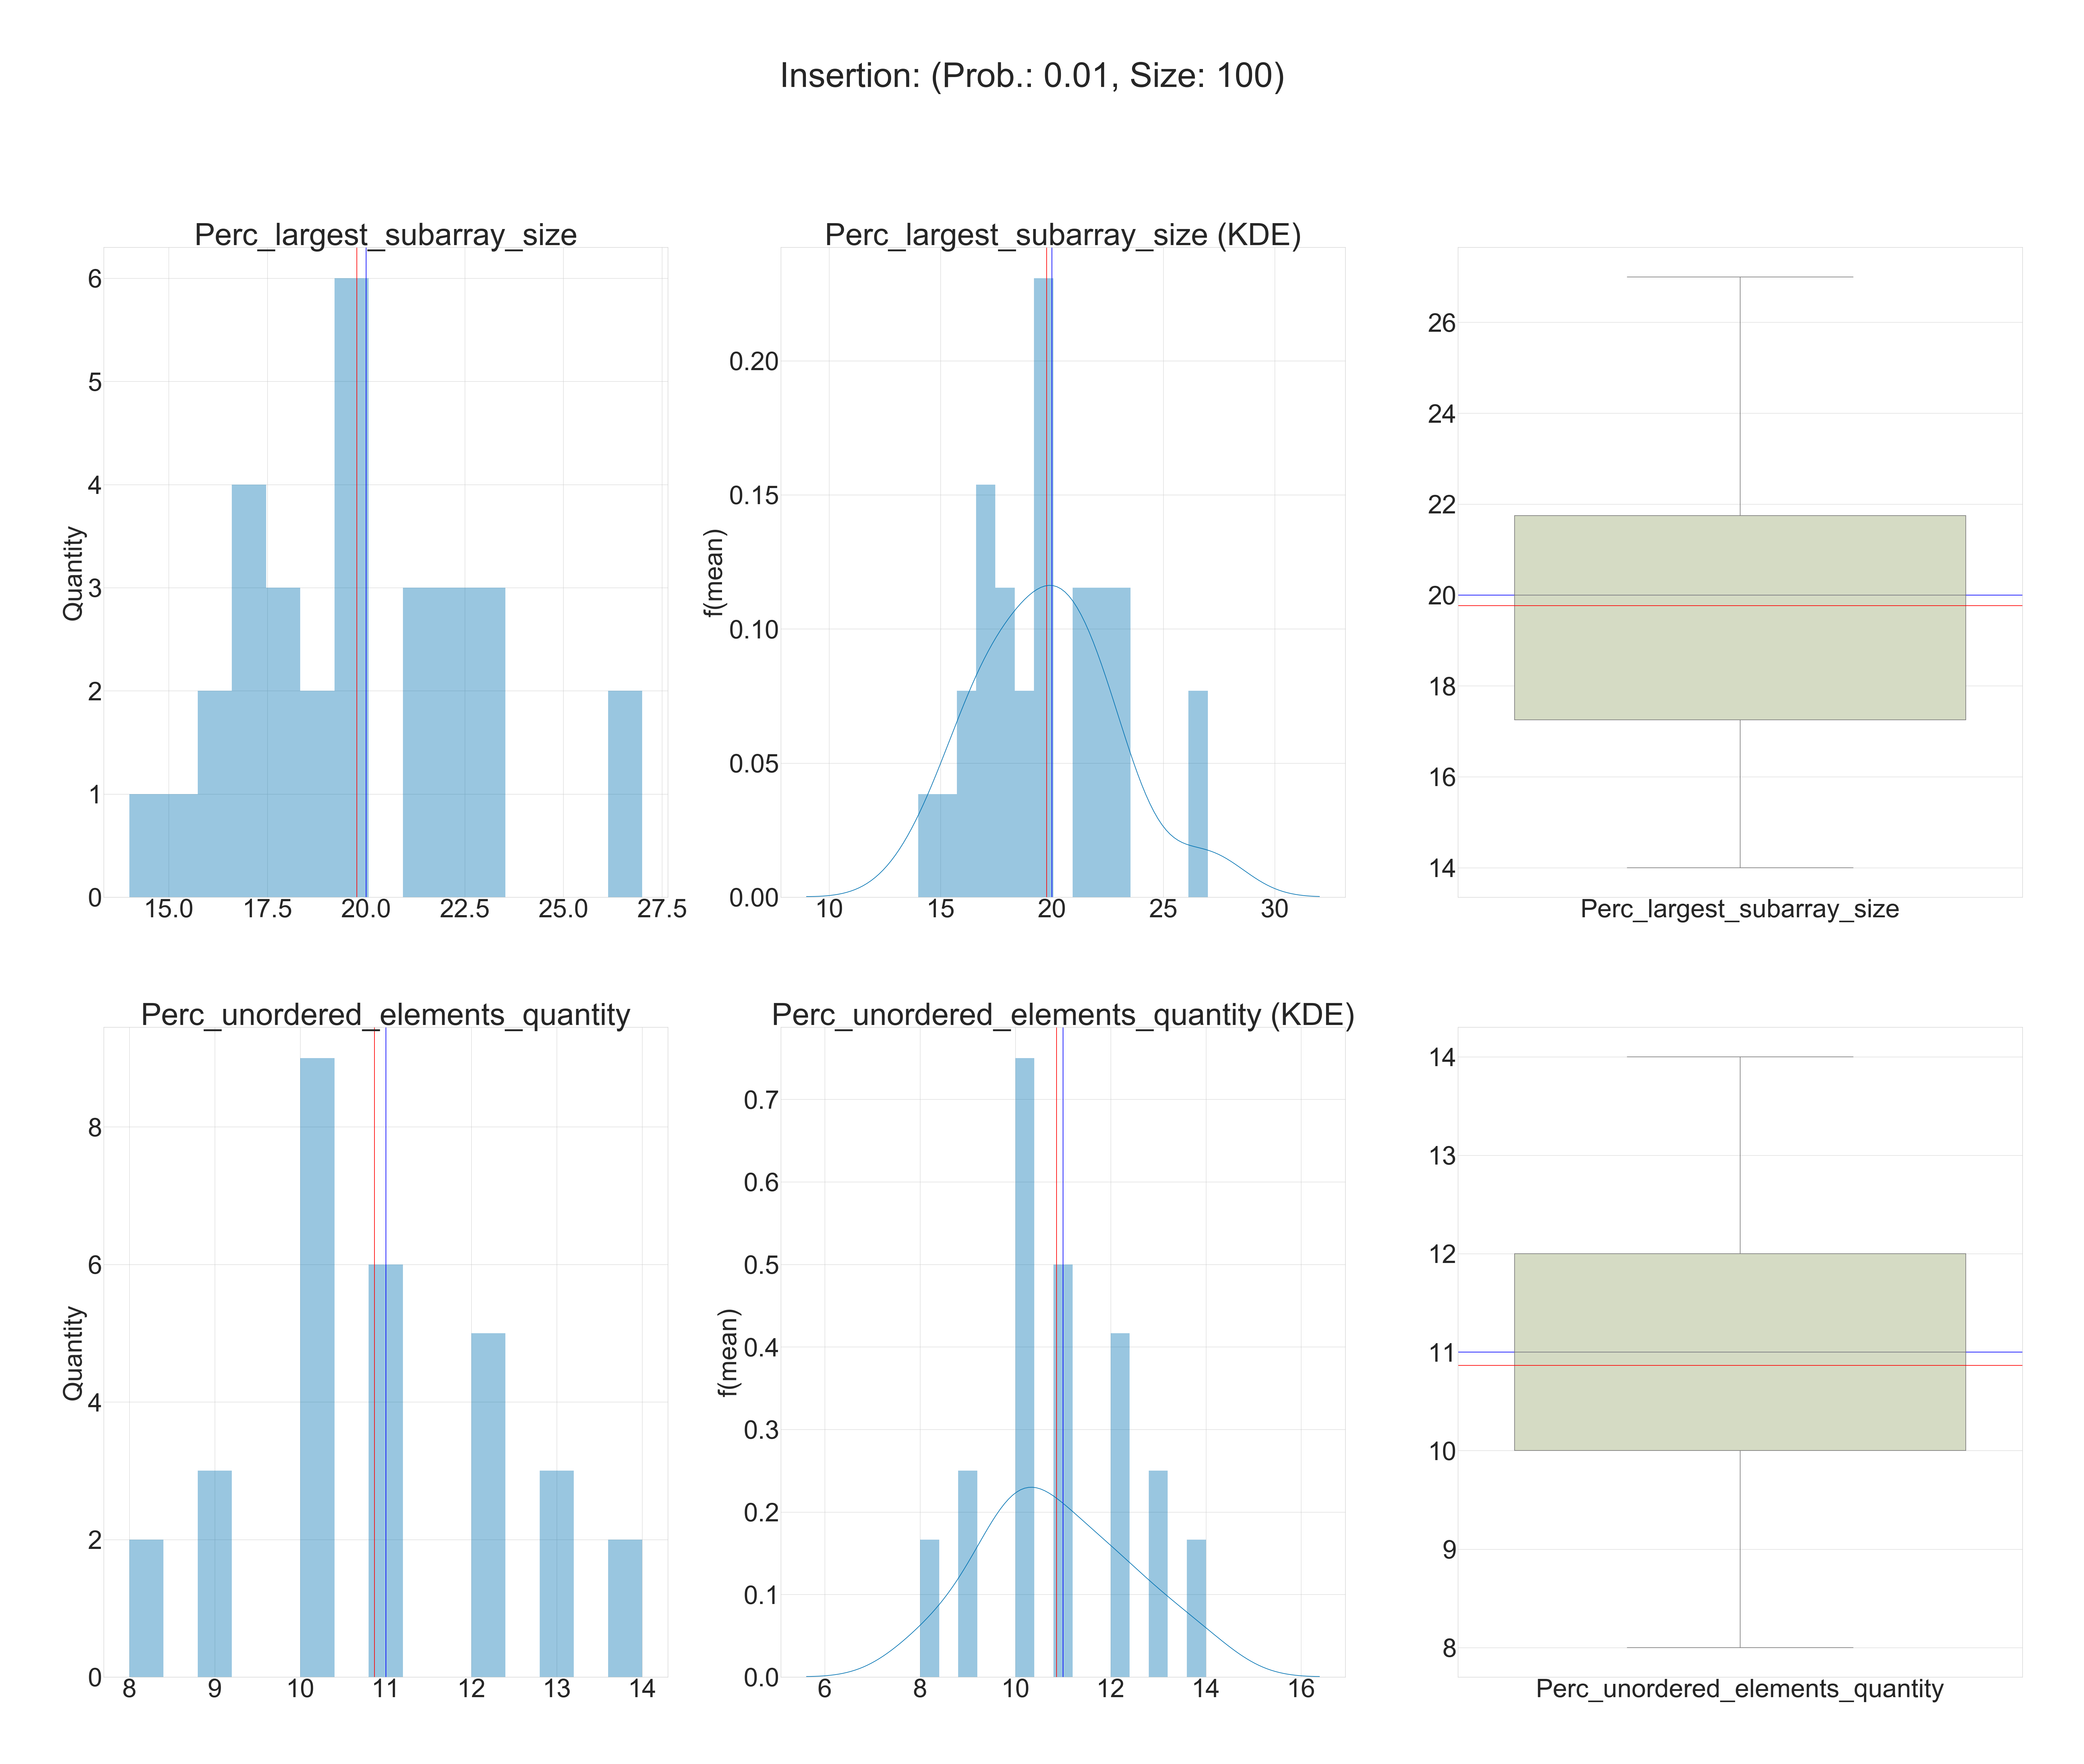
\includegraphics[scale=0.105]{figures/0_01_100_Insertion.png}}
    \caption{Histograms and Boxplot for Insertion sort, with \textit{probability of failure} of 0.01 and \textit{array size} of 100.}
    \label{fig-histogram-boxplot-insertion-001100}
\end{figure}

\begin{figure}[H]
    \centering
    \frame{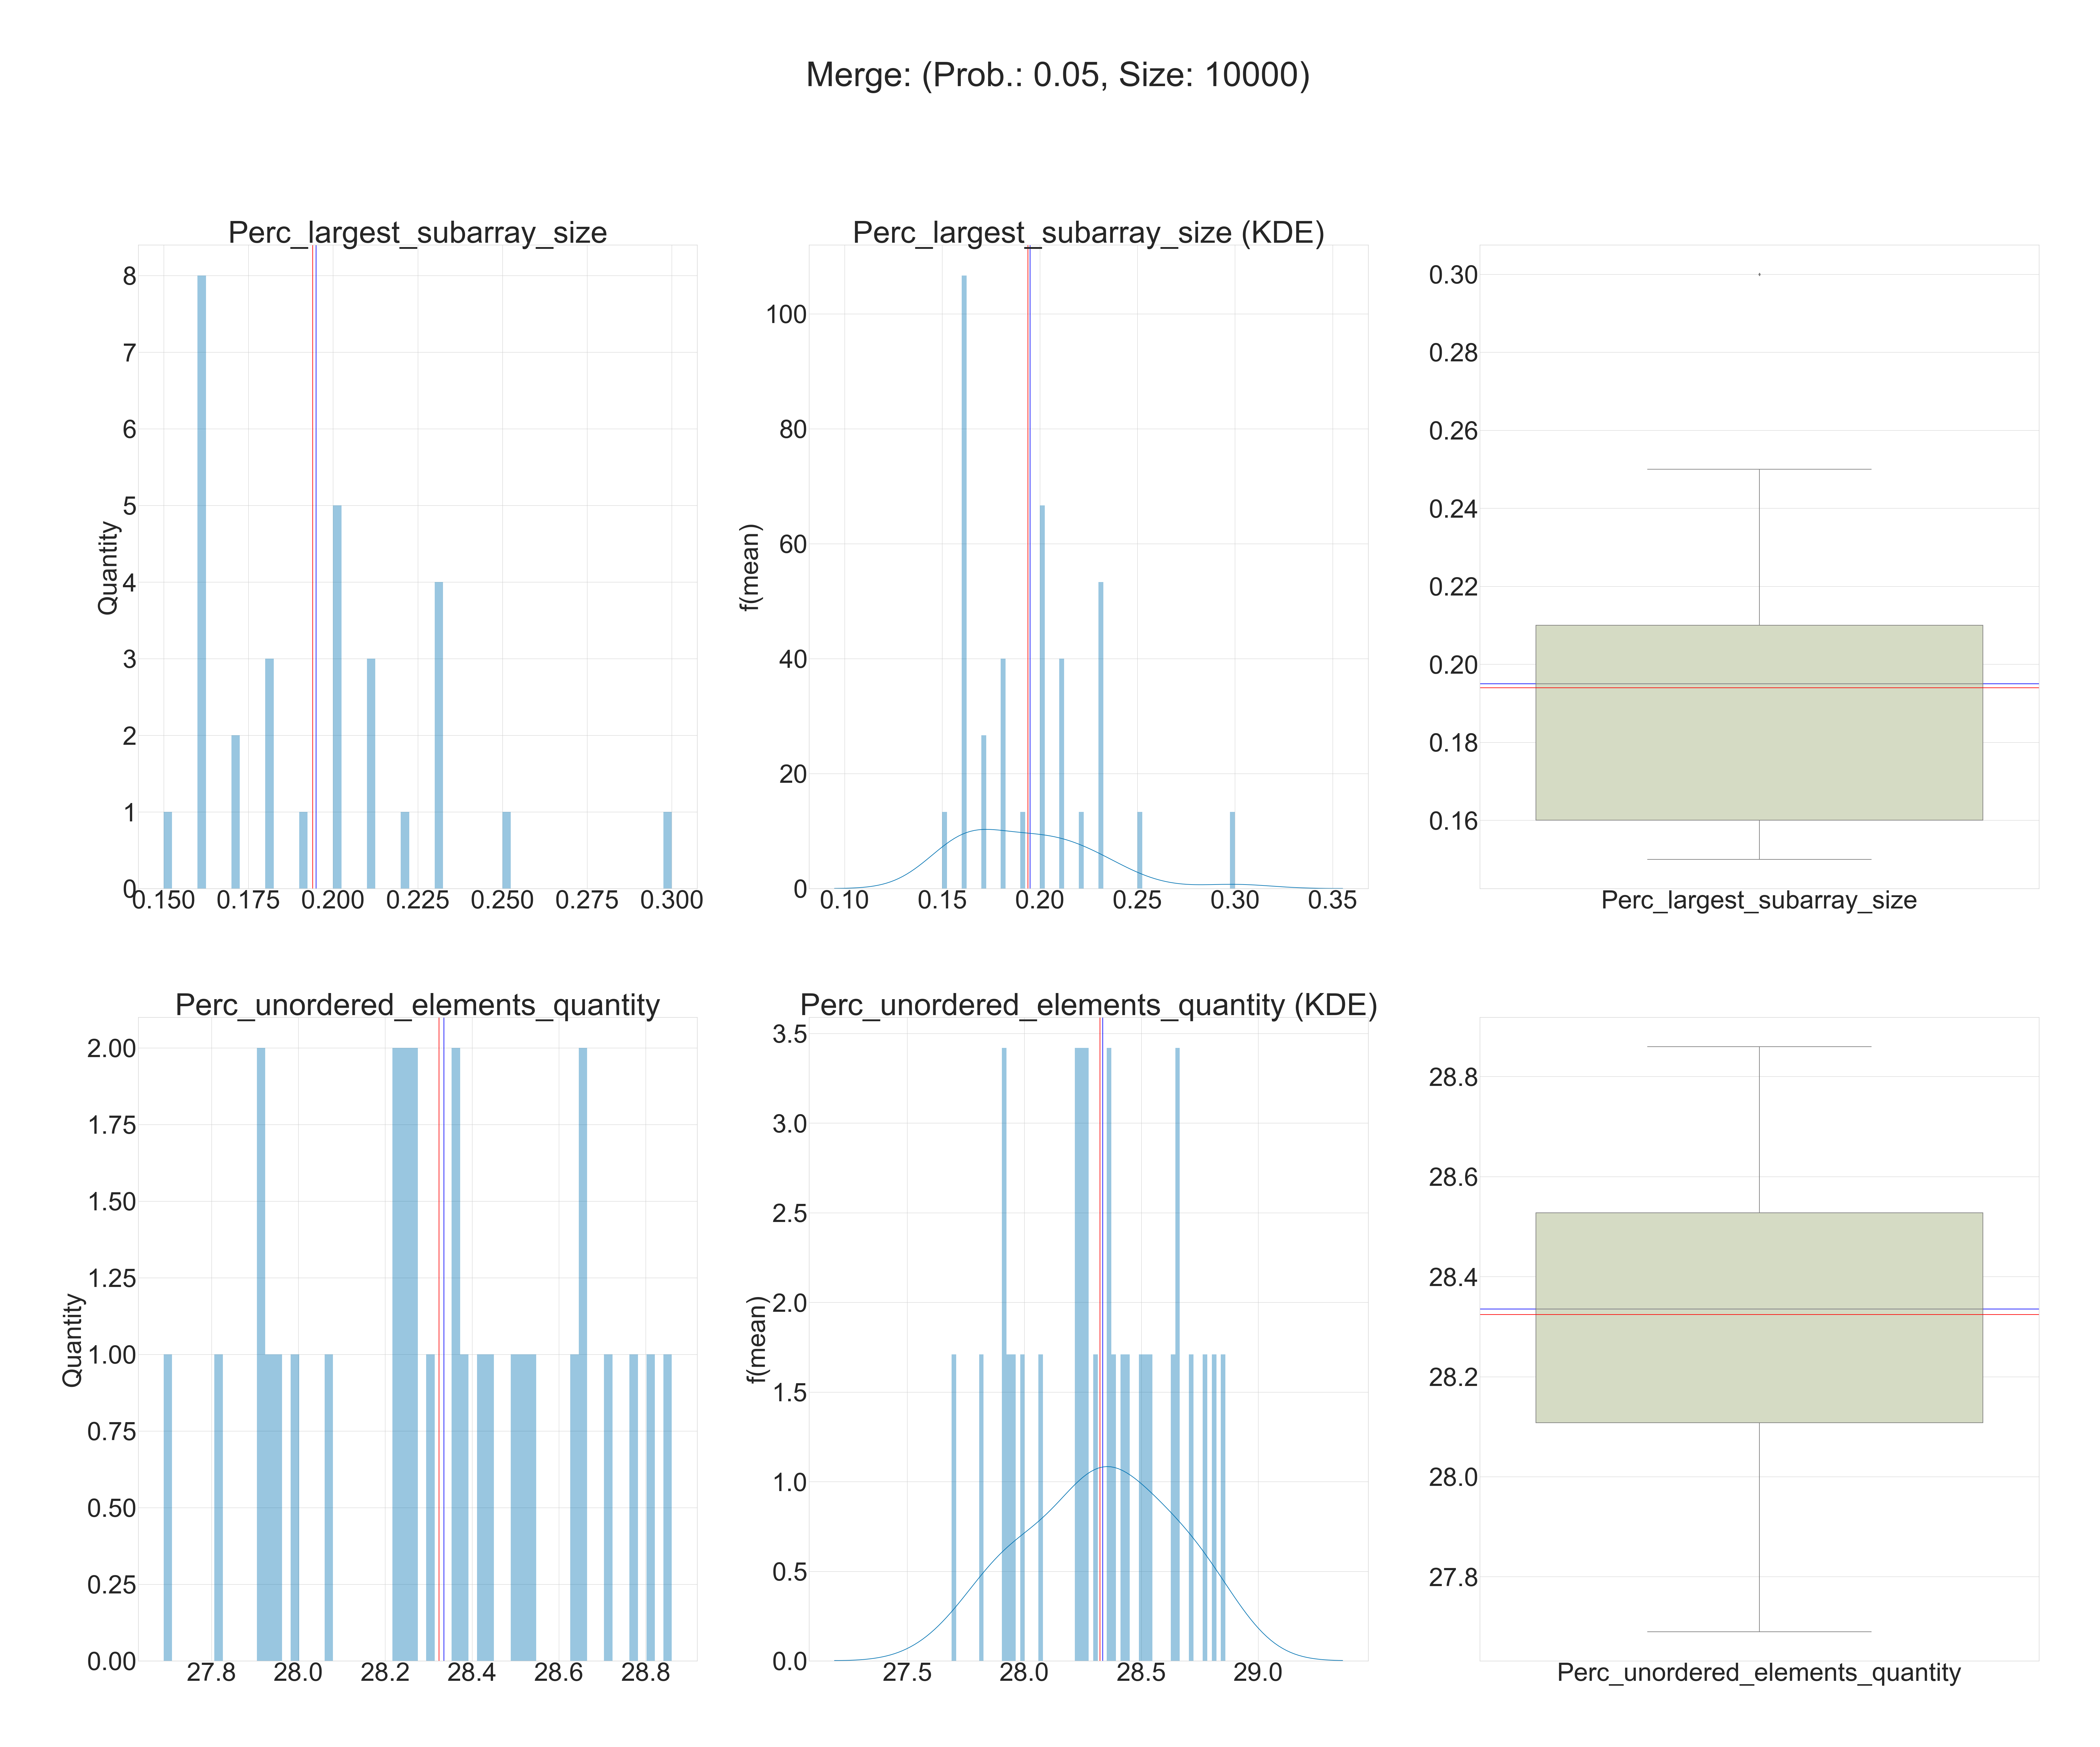
\includegraphics[scale=0.105]{figures/0_05_10000_Merge.png}}
    \caption{Histograms and Boxplot for Mergesort, with \textit{probability of failure} of 0.05 and \textit{array size} of 10000.}
    \label{fig-histogram-boxplot-merge-00510000}
\end{figure}

\begin{figure}[H]
    \centering
    \frame{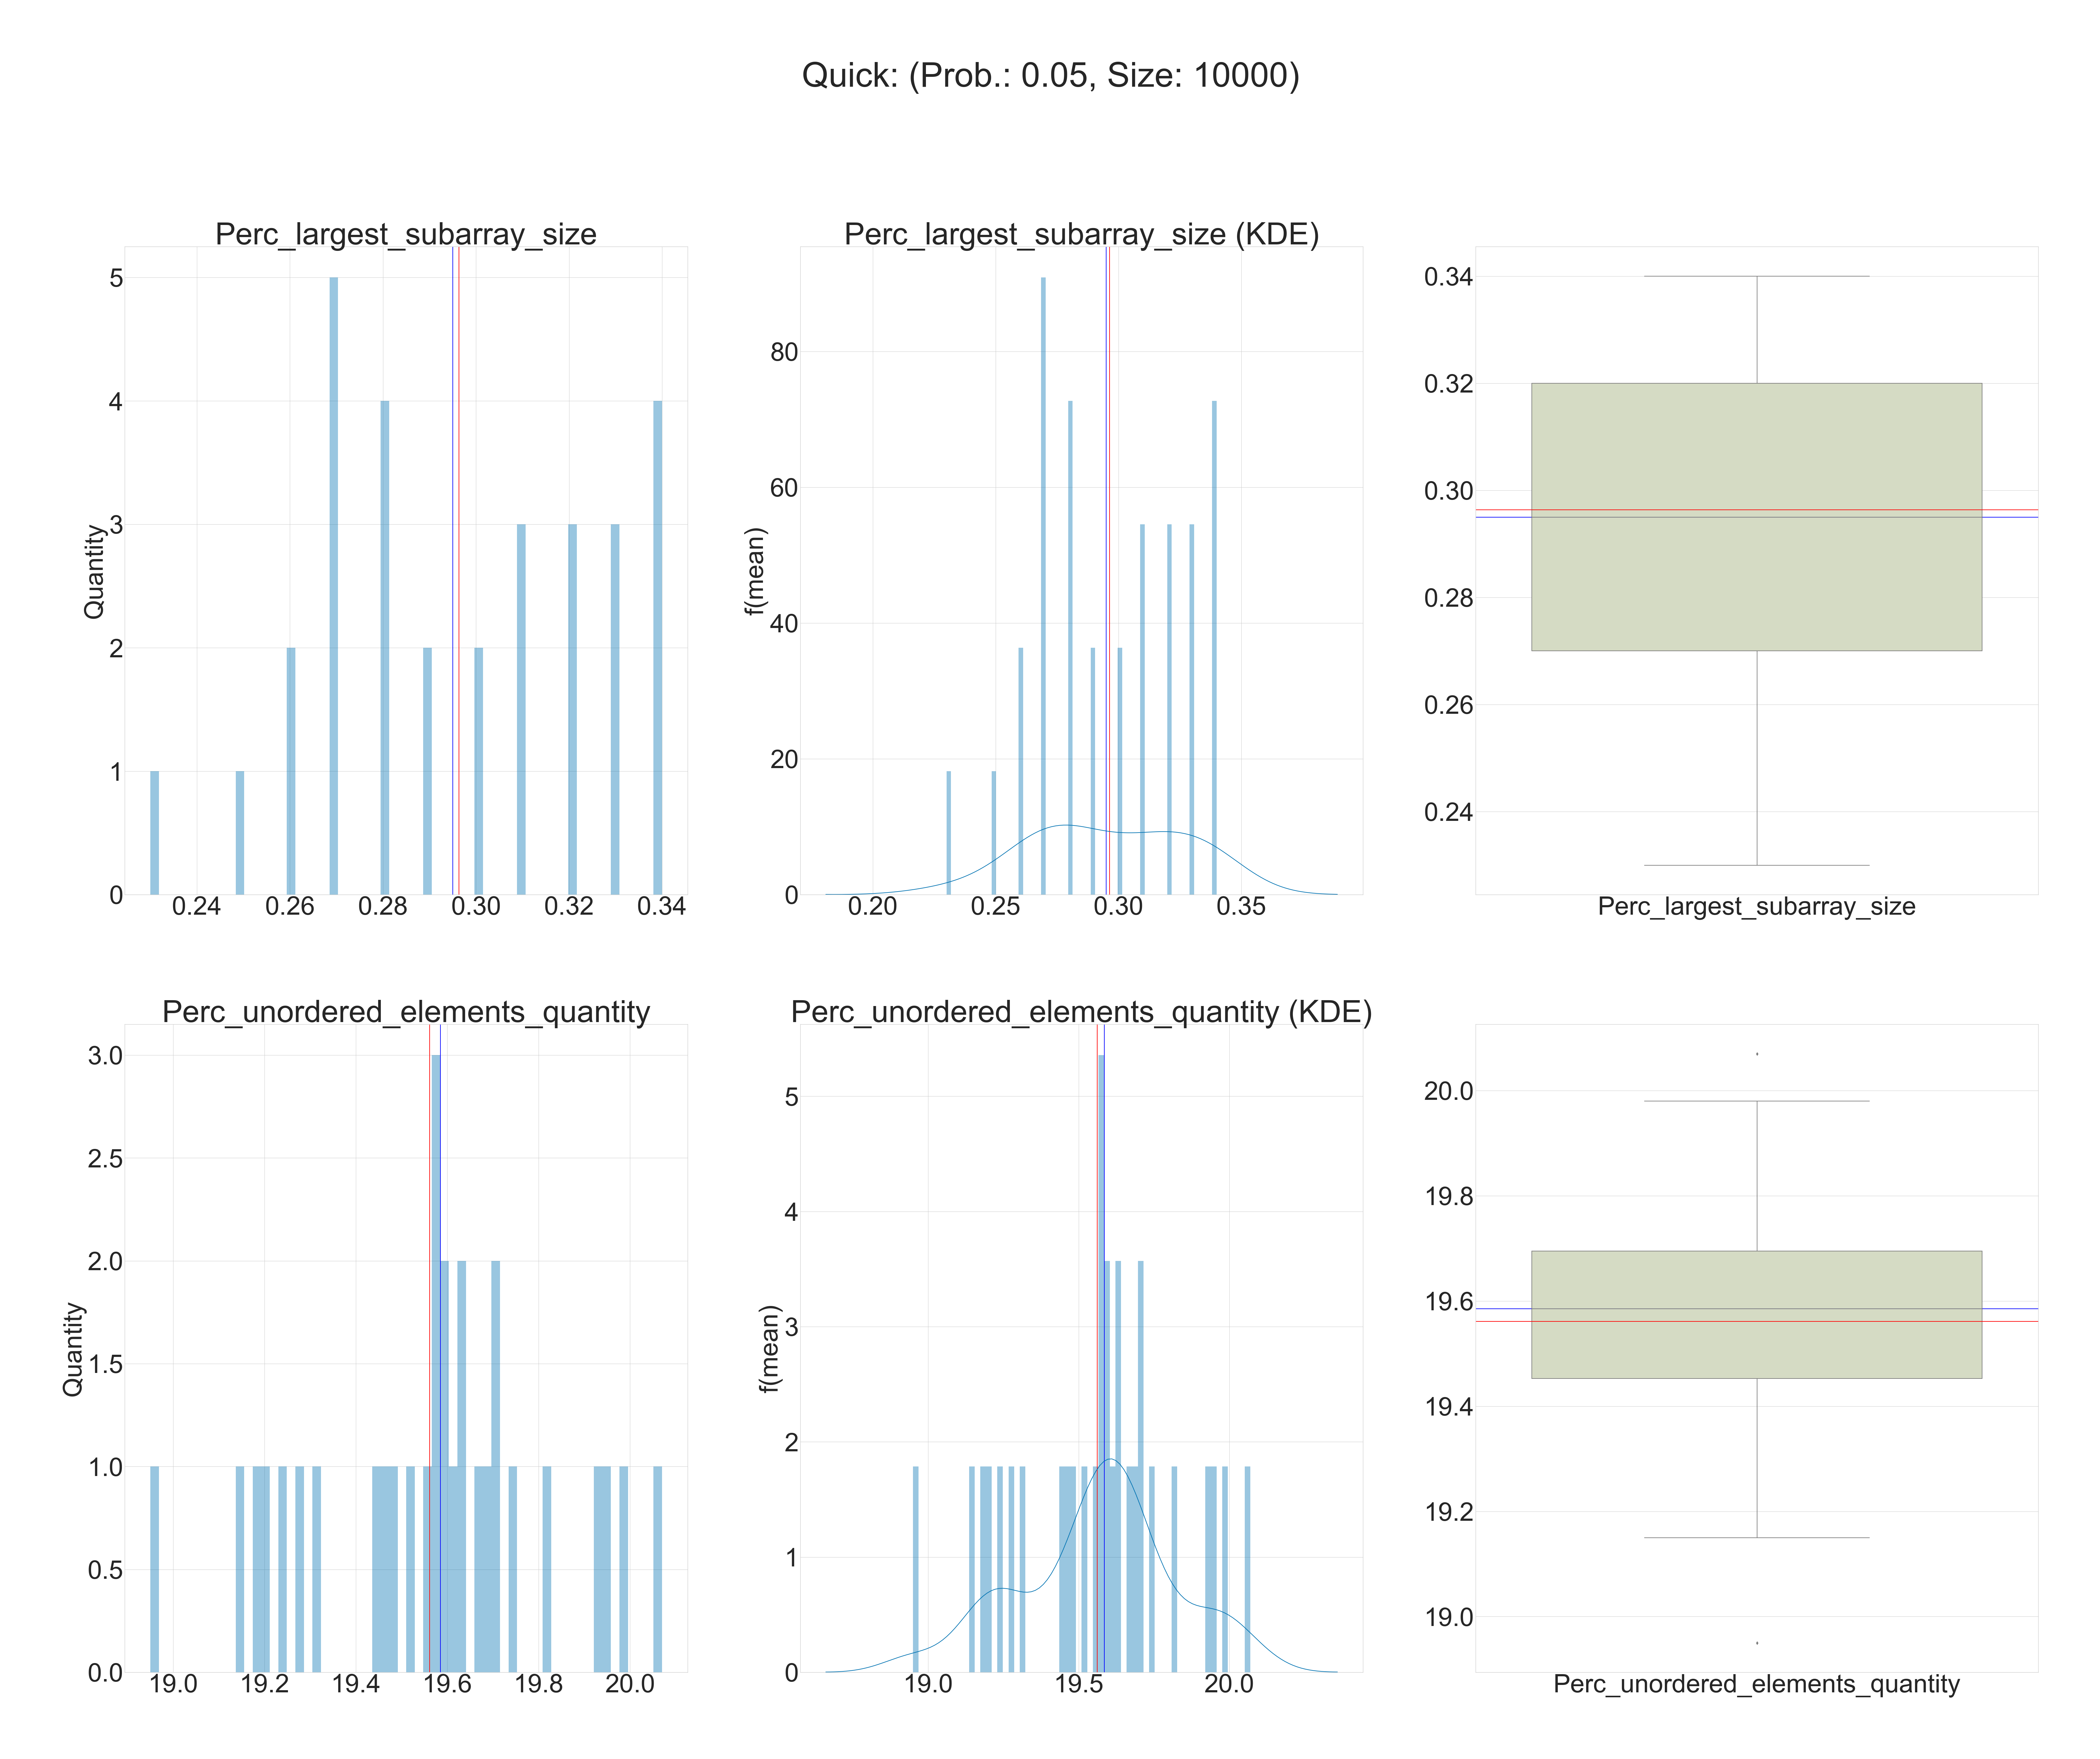
\includegraphics[scale=0.105]{figures/0_05_10000_Quick.png}}
    \caption{Histograms and Boxplot for Quicksort, with \textit{probability of failure} of 0.05 and \textit{array size} of 10000.}
    \label{fig-histogram-boxplot-quick-00510000}
\end{figure}

We produced graphs with the same data about dependent variables showed in tables before. Figure X shows an example of these graphs.